\documentclass[../main.tex]{subfiles}
\graphicspath{{\subfix{../images/}}}

\begin{document}


\subsection{Data Description}

The data set we are using for this project is a subset of the 
fashion MNIST data set. It contains $15$,$000$ $28 \times 28$ 
grey-scale images, that are represented as flattened arrays and is 
pre-split into two data sets -- a training data set with $10$,$000$ 
images and a test data set with $5$,$000$ images and their 
associated labels. 

\begin{figure}[ht]
    \centering
    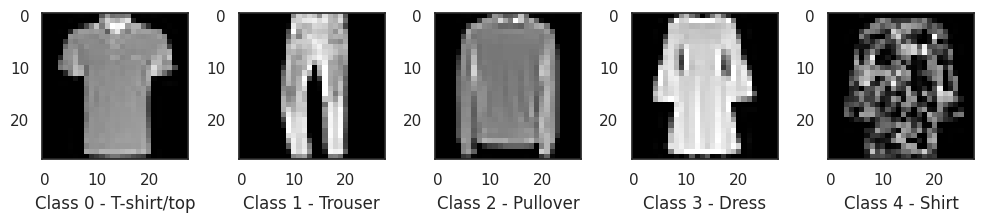
\includegraphics[width=\textwidth]
    {images/clothing_image_report.png}
    \caption{A random sample from the training set of 5 images one 
    from each class}
    \label{fig:clothes}
\end{figure}

Each image has a total of $784$ pixels and each pixel has an 
associated pixel-value that ranges from $0$ to $255$, which 
represents the brightness of the pixel. 
Each image has been assigned one of 5 labels, to encode which 
article of clothing the image is of (\autoref{tab:label_enc}).

\begin{table}[ht]
    \centering
    \rowcolors{2}{white}{white}
    \begin{tabular}{lccccc}
\hline Type of clothing & T-shirt/top & Trouser & Pullover & Dress & Shirt \\
\hline Label & 0 & 1 & 2 & 3 & 4 \\
\hline
\end{tabular}
    \caption{Label encoding}
    \label{tab:label_enc}
\end{table}


\subsection{Data Cleaning}

We carried out some different integrity checks of the data. Such as 
checking for missing values, ensuring values are integers only and 
in the correct range i.e. pixel-values between $0$ and $255$ and 
labels between $0$ and $4$. We didn't find any inconsistencies, and 
therefore no data cleaning was needed. 


\end{document}